\documentclass[tikz,border=2pt]{standalone}
\usepackage{amsmath,amssymb}
\usepackage{tikz}
\usetikzlibrary{arrows.meta}

\begin{document}
% An integer linear program keeps the linear objective and constraints but allows only
% integer points: the feasible set is a set of isolated dots, not a polygon, so corner-point
% reasoning and the simplex method no longer apply directly.
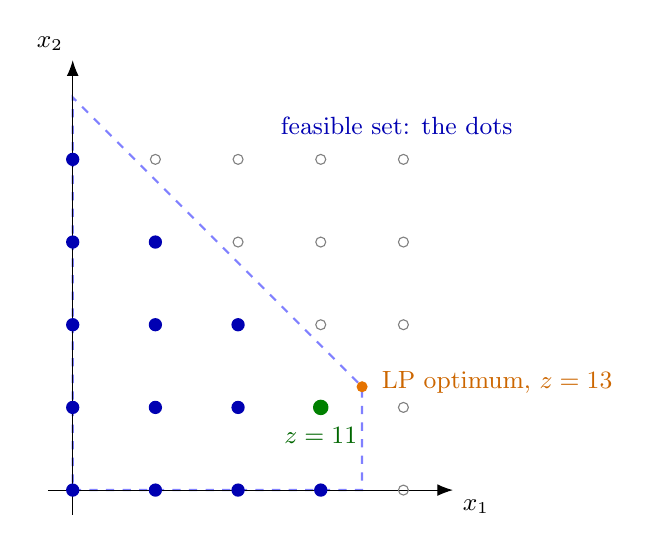
\begin{tikzpicture}[x=1.05cm, y=1.05cm, every node/.style={font=\small}, >={Latex[length=2mm]}]
	\draw[blue!50, thick, dashed] (0,0) -- (3.5,0) -- (3.5,1.25) -- (0,4.75) -- cycle;
	\draw[->] (-0.3,0) -- (4.6,0) node[below right] {$x_1$};
	\draw[->] (0,-0.3) -- (0,5.2) node[above left] {$x_2$};
	\foreach \i in {0,1,2,3,4} {\foreach \j in {0,1,2,3,4} {
		\pgfmathparse{(2*\i+2*\j<=9.5 && \i<=3.5) ? 1 : 0}
		\ifnum\pgfmathresult=1 \fill[blue!70!black] (\i,\j) circle (2.4pt); \else \draw[gray] (\i,\j) circle (1.8pt); \fi
	}}
	\fill[orange!90!black] (3.5,1.25) circle (2pt);
	\node[orange!80!black, anchor=west] at (3.62,1.3) {LP optimum, $z=13$};
	\fill[green!50!black] (3,1) circle (2.8pt);
	\node[green!40!black, anchor=north] at (3,0.88) {$z=11$};
	\node[blue!70!black, font=\small, anchor=west] at (2.4,4.4) {feasible set: the dots};
	\end{tikzpicture}
\end{document}
